\chapter{Envisioned Approach}
\begin{figure}[H]
  \centering
  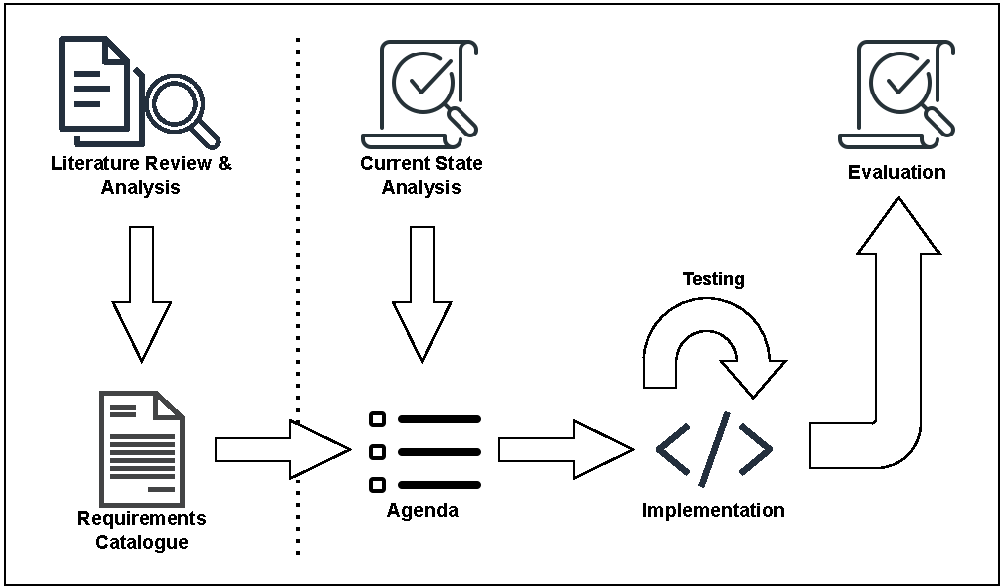
\includegraphics[width=0.75\textwidth]{img/approach_figure.pdf}
  \caption{Approach of the Thesis}
  \label{fig:approach_figure}
\end{figure}

Figure \ref{fig:approach_figure} visualises the general approach of the thesis showing distinct steps to meet the goals of the thesis.
First the state of art is determined, which is neatly followed by an analysis to determine the requirements catalogue (\ref{approach:state-of-art}).
Then, Ecoscape is analyzed to have a comparable base to the content of the catalogue (\ref{approach:ecoscape-current-state}) and based on that comparison the implementation takes place (\ref{approach:ecoscape-implementation}).
At the end an evaluation of Ecoscape takes place (\ref{approach:ecoscape-evaluation}).
\\
In the following sections, each step is further described.
\section{State of Art and Requirements Catalogue}\label{approach:state-of-art}
The computing simulation landscape is vast with different simulators, which can have all different bias, metrics, implementations, use-cases, focus and features.
There are for example pure edge computing simulators like EdgeSim++ [\cite{10612841}] or EdgeCloudSim [\cite{10.1002/ett.3493}] , pure fog computing simulators like iFogSim [\cite{gupta2016ifogsimtoolkitmodelingsimulation}] or YAFS [\cite{8758823}] and hybrid variants like PureEdgeSim [\cite{9188059}] or FogNetSim++ [\cite{8502760}].

To have a common ground, we firstly use literature review to compute a list of simulators that we deem state of art based on the general consens of the edge computing landscape.
We further determine their respective quality characteristics, use-cases, focus and approach through said literature review and with further testing a broader knowledge about each simulator can be determined.
This testing can be done by running the simulators with the same use-cases, testbeds like presented by \cite{pfandzelter2024lessonslearnedbuildingedge} and subsequently comparing the results.
This gives us a good overview of the current state of art simulators and their respective strengths and weaknesses as well as their similarities and differences.
Based on the results of the literature review and the testing, we then can construct a requirements catalogue that defines the necessary and optional features, metrics and characteristics of a proper edge computing simulator.

\section{Ecoscape}\label{approach:ecoscape}
\subsection{Analysis of current state}\label{approach:ecoscape-current-state}
To advance Ecoscape, we firstly need to determine Ecoscape's strengths and weaknesses in comparison to the requirements catalogue. 
Therefore in a similar manner as we reviewed and tested the state of art simulators in section \ref{approach:state-of-art}, we need to review and test Ecoscape.
We then can compare the resulting points with the catalogue to determine the set of requirements that Ecoscape currently meets and some where it underperforms.
This gives us an agenda for the next step.

\subsection{Implementation}\label{approach:ecoscape-implementation}
Based on the result of section \ref{approach:ecoscape-current-state}, the currently good and bad points of ecoscape should be clear. This step therefore is focusing on implementing missing features as well as improving existing features 
to meet the requirements catalogue.
The implementation will be done part of the Ecoscape project and therefore should be good documented as well as steadily tested to guarantee satisfying results. 

\subsection{Evaluation}\label{approach:ecoscape-evaluation}
At the end, an evaluation takes place to determine if the resulting version of Ecoscape is meeting expectations. At this point the evaluation should take place over multiple use-cases and will be done via user study or expert interviews.
The exact parameters of said evaluation still need to be defined.